\documentclass{beamer}
\usepackage[utf8]{inputenc}
\usepackage{hyperref}
\usepackage{multicol}
\usepackage{hyperref}
\usepackage{amsmath}
\usepackage[english]{babel}
\usepackage{algorithm}
\usepackage[noend]{algpseudocode}

\inputencoding{utf8}

\mode<presentation> {
    \usetheme{Madrid}
}

\usepackage{graphicx}
\usepackage{booktabs}

\title[Codiciosos]{Algoritmos Codiciosos}
\author{Ernesto Rodriguez - Juan Roberto Alvaro Saravia}
\institute{
    Universidad Francisco Marroquin \\
    \medskip \textit{ernestorodriguez@ufm.edu - juanalvarado@ufm.edu}
}

\date[\today]{}

\begin{document}

\begin{frame}
\titlepage
\end{frame}

\begin{frame}
\frametitle{Cordinaci\'on de Actividades}
\begin{itemize}
\item{Se tiene un conjunto de actividades $A=\{a_1,a_2,\ldots,a_n\}$}
\item{Las actividades hacen uso de un recurso comun.}
\item{Toda actividad tiene una hora de inicio ($t_0$) y
    hora de finalizaci\'on ($t_f$).}
\item{Dos actividades $a_1,a_2\in A$ son {\bf compatibles} si
    los intervalos $[t_0^{a_1},t_f^{a_1})$ y $[t_0^{a_2},t_f^{a_2})$
    no traslapan.}
\item{Las actividades $a_1,a_2,\ldots,a_n$ se encuentran ordenadas
    de forma ascendiente respecto a $t_f$, es decir: $t_f^{a_1}\leq
    t_f^{a_2}\leq\ldots\leq t_f^{a_n}$}
\end{itemize}
{\bf Problema: } Encontrar el subconjunto $A_c\subset A$ con la
mayor cantidad de {\bf actividades compatibles}.
\end{frame}

\begin{frame}
\frametitle{Cordinaci\'on de Actividades}
\begin{center}
    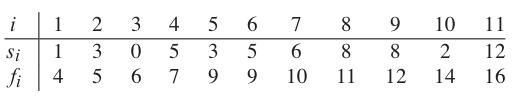
\includegraphics[width=10cm]{./actividades.png}
\end{center}
Actividades compatibles:\\
\begin{itemize}
    \item{$\{a_3,a_9,a_{11}\}$}
    \item{$\{a_1,a_4,a_8,a_{11}\}$}
    \item{$\{a_2,a_4,a_9,a{11}\}$}
\end{itemize}
\end{frame}

\begin{frame}
\frametitle{Programaci\'on Dinamica (idea)}
\begin{algorithm}[H]
    \caption{Cordinar}
    \begin{algorithmic}[1]
    \Procedure{Cordinar}{$t_0,t_f,A$}
    \State{{\bf let}\ $A_c=\{\}$}
    \For{$a_i$ {\bf in} A}
        \State{{\bf let} $opcion=\{\}$}
        \If{$[t_0^{a_i},t_f^{a_i})\subseteq [t_0,t_f)$}
            \State{{\bf let} $resto=A\backslash \{a_i\}$}
            \State{{\bf let} $opcion_0=\mathtt{Cordinar}(t_0,t_0^{a_i}, resto)$}
            \State{{\bf let} $opcion_f=\mathtt{Cordinar}(t_f^{a_i},t_f, resto)$}
            \State{$opcion\gets \{a_i\}\cup opcion_0\cup opcion_f$}
            \State{$A_c\gets \mathtt{mayor}(A_c,opcion)$}
        \EndIf
    \EndFor
    \State{{\bf return} $A_c$}
    \EndProcedure
    \end{algorithmic}
\end{algorithm}
\end{frame}

\begin{frame}
\frametitle{Programaci\'on Dinamica}
\begin{itemize}
    \item{El algoritmo hace uso de la memorizaci\'on para
    evitar repetir trabajo.}
    \item{Sin embargo, ¿es necesario considerar todas las
    opciones?}
    \item{¿Se puede decidir si agregar o no una actividad
    sin tener que resolver todos los sub-problemas?}
\end{itemize}
\end{frame}

\begin{frame}
\frametitle{Seleci\'on Codiciosa}
\begin{itemize}
    \item{Seleccionar la actividad que deje la mayor
    cantidad de tiempo libre.}
    \item{En otras palabras, seleccionar la actividad
    que termine lo m\'as temprano posible.}
    \item{En caso de conflicto, hacer una seleci\'on
    arbitraria.}
\end{itemize}
\end{frame}

\begin{frame}
\frametitle{Algoritmos Codiciosos}
\begin{itemize}
    \item{La programaci\'on dinamica es una herramienta poderosa
    ya que considera un amplio espacio de combinaciones.}
    \item{Sin embargo, existen ocasiones en que la programaci\'on
    dinamica es un metodo ``exagerado''.}
    \item{Ciertos problemas pueden ser resuletos seleccionando
    la opci\'on optima en cada paso, sin importar como se
    desenvuelba el resto de la busqueda.}
    \item{A estos algoritmos se les conoce como {\bf algoritmos
    codiciosos}.}
\end{itemize}
\end{frame}

\begin{frame}
\frametitle{Creaci\'on de Algoritmos Codiciosos}
\begin{enumerate}
    \item{Encontrar la sub-estructura optima}
    \item{Crear una soluci\'on recursiva que busque esa sub-estructura}
    \item{Demostrar que al hacer la elecci\'on codiciosa,
    solamente queda un sub-problema}
    \item{Demostrar que es ``seguro'' hacer la soluci\'on codiciosa}
    \item{Implementar el algoritmo recursivamente}
    \item{Implementar el algoritmo iterativamente}
\end{enumerate}
\end{frame}

\begin{frame}
\frametitle{Elecciones codiciosas vs Programaci\'on dinamica}
\begin{itemize}
    \item{Las decisiones codiciosas solo consideran el ``pasado'',
    mientras la programaci\'on dinamica considera tambien el ``futuro''}
    \item{La programaci\'on dinamica es m\'as general que los
    algoritmos codiciosos.}
    \item{Los algoritmos codiciosos son m\'as eficientes.}
    \item{En algunas ocasiones, agregarle restricciones a un problema
    permite utilizar algoritmos codiciosos:
        \begin{itemize}
            \item{TSP vs Shortest Path}
            \item{Candelarizaci\'on vs Candelarizaci\'on Generalizada}
            \item{Ordenamiento vs Ordenamiento Generalizado}
            \item{Knapsack fracionado vs Knapsack con Limite vs Knapsack Generalizado}
        \end{itemize}}
\end{itemize}
\end{frame}

\end{document}